% =====================================================================
%  Front cover — Is the Riemann Hypothesis Solved?
%  Typeset standalone at the 6 x 9 in trim, full bleed.
%  Vertical positions are in inches measured from the foot of the page and
%  are given as baselines, matching the plate's own composition.
% =====================================================================
\documentclass{article}
\usepackage[paperwidth=6in,paperheight=9in,margin=0pt]{geometry}
\usepackage{fontspec}
\usepackage{xcolor}
\usepackage{graphicx}
\usepackage{tikz}

\setmainfont{Outfit}[
  UprightFont={Outfit Regular}, BoldFont={Outfit Bold},
  ItalicFont={Outfit Regular}, ItalicFeatures={FakeSlant=0.20},
  BoldItalicFont={Outfit Bold}, BoldItalicFeatures={FakeSlant=0.20},
  Ligatures={TeX}]
% The cover sets most of its type in \sffamily. Without an explicit
% sans face that is Latin Modern Sans, so the cover would carry two
% typefaces where the book carries one.
\setsansfont{Outfit}[
  UprightFont={Outfit Regular}, BoldFont={Outfit Bold},
  ItalicFont={Outfit Regular}, ItalicFeatures={FakeSlant=0.20},
  BoldItalicFont={Outfit Bold}, BoldItalicFeatures={FakeSlant=0.20},
  Ligatures={TeX}]
\setmonofont{DejaVu Sans Mono}[
  UprightFont={DejaVu Sans Mono}, BoldFont={DejaVu Sans Mono Bold},
  Ligatures={TeX}]

\definecolor{ink}{HTML}{0C1016}
\definecolor{accent}{HTML}{8FD6C0}
\definecolor{txt}{HTML}{E6EBEF}
\definecolor{dim}{HTML}{8B9BA7}

\pagestyle{empty}
\setlength{\parindent}{0pt}


\begin{document}
\begin{tikzpicture}[remember picture,overlay]
  % ---- the plate, full bleed --------------------------------------------
  \node[anchor=south west,inner sep=0] at (current page.south west)
    {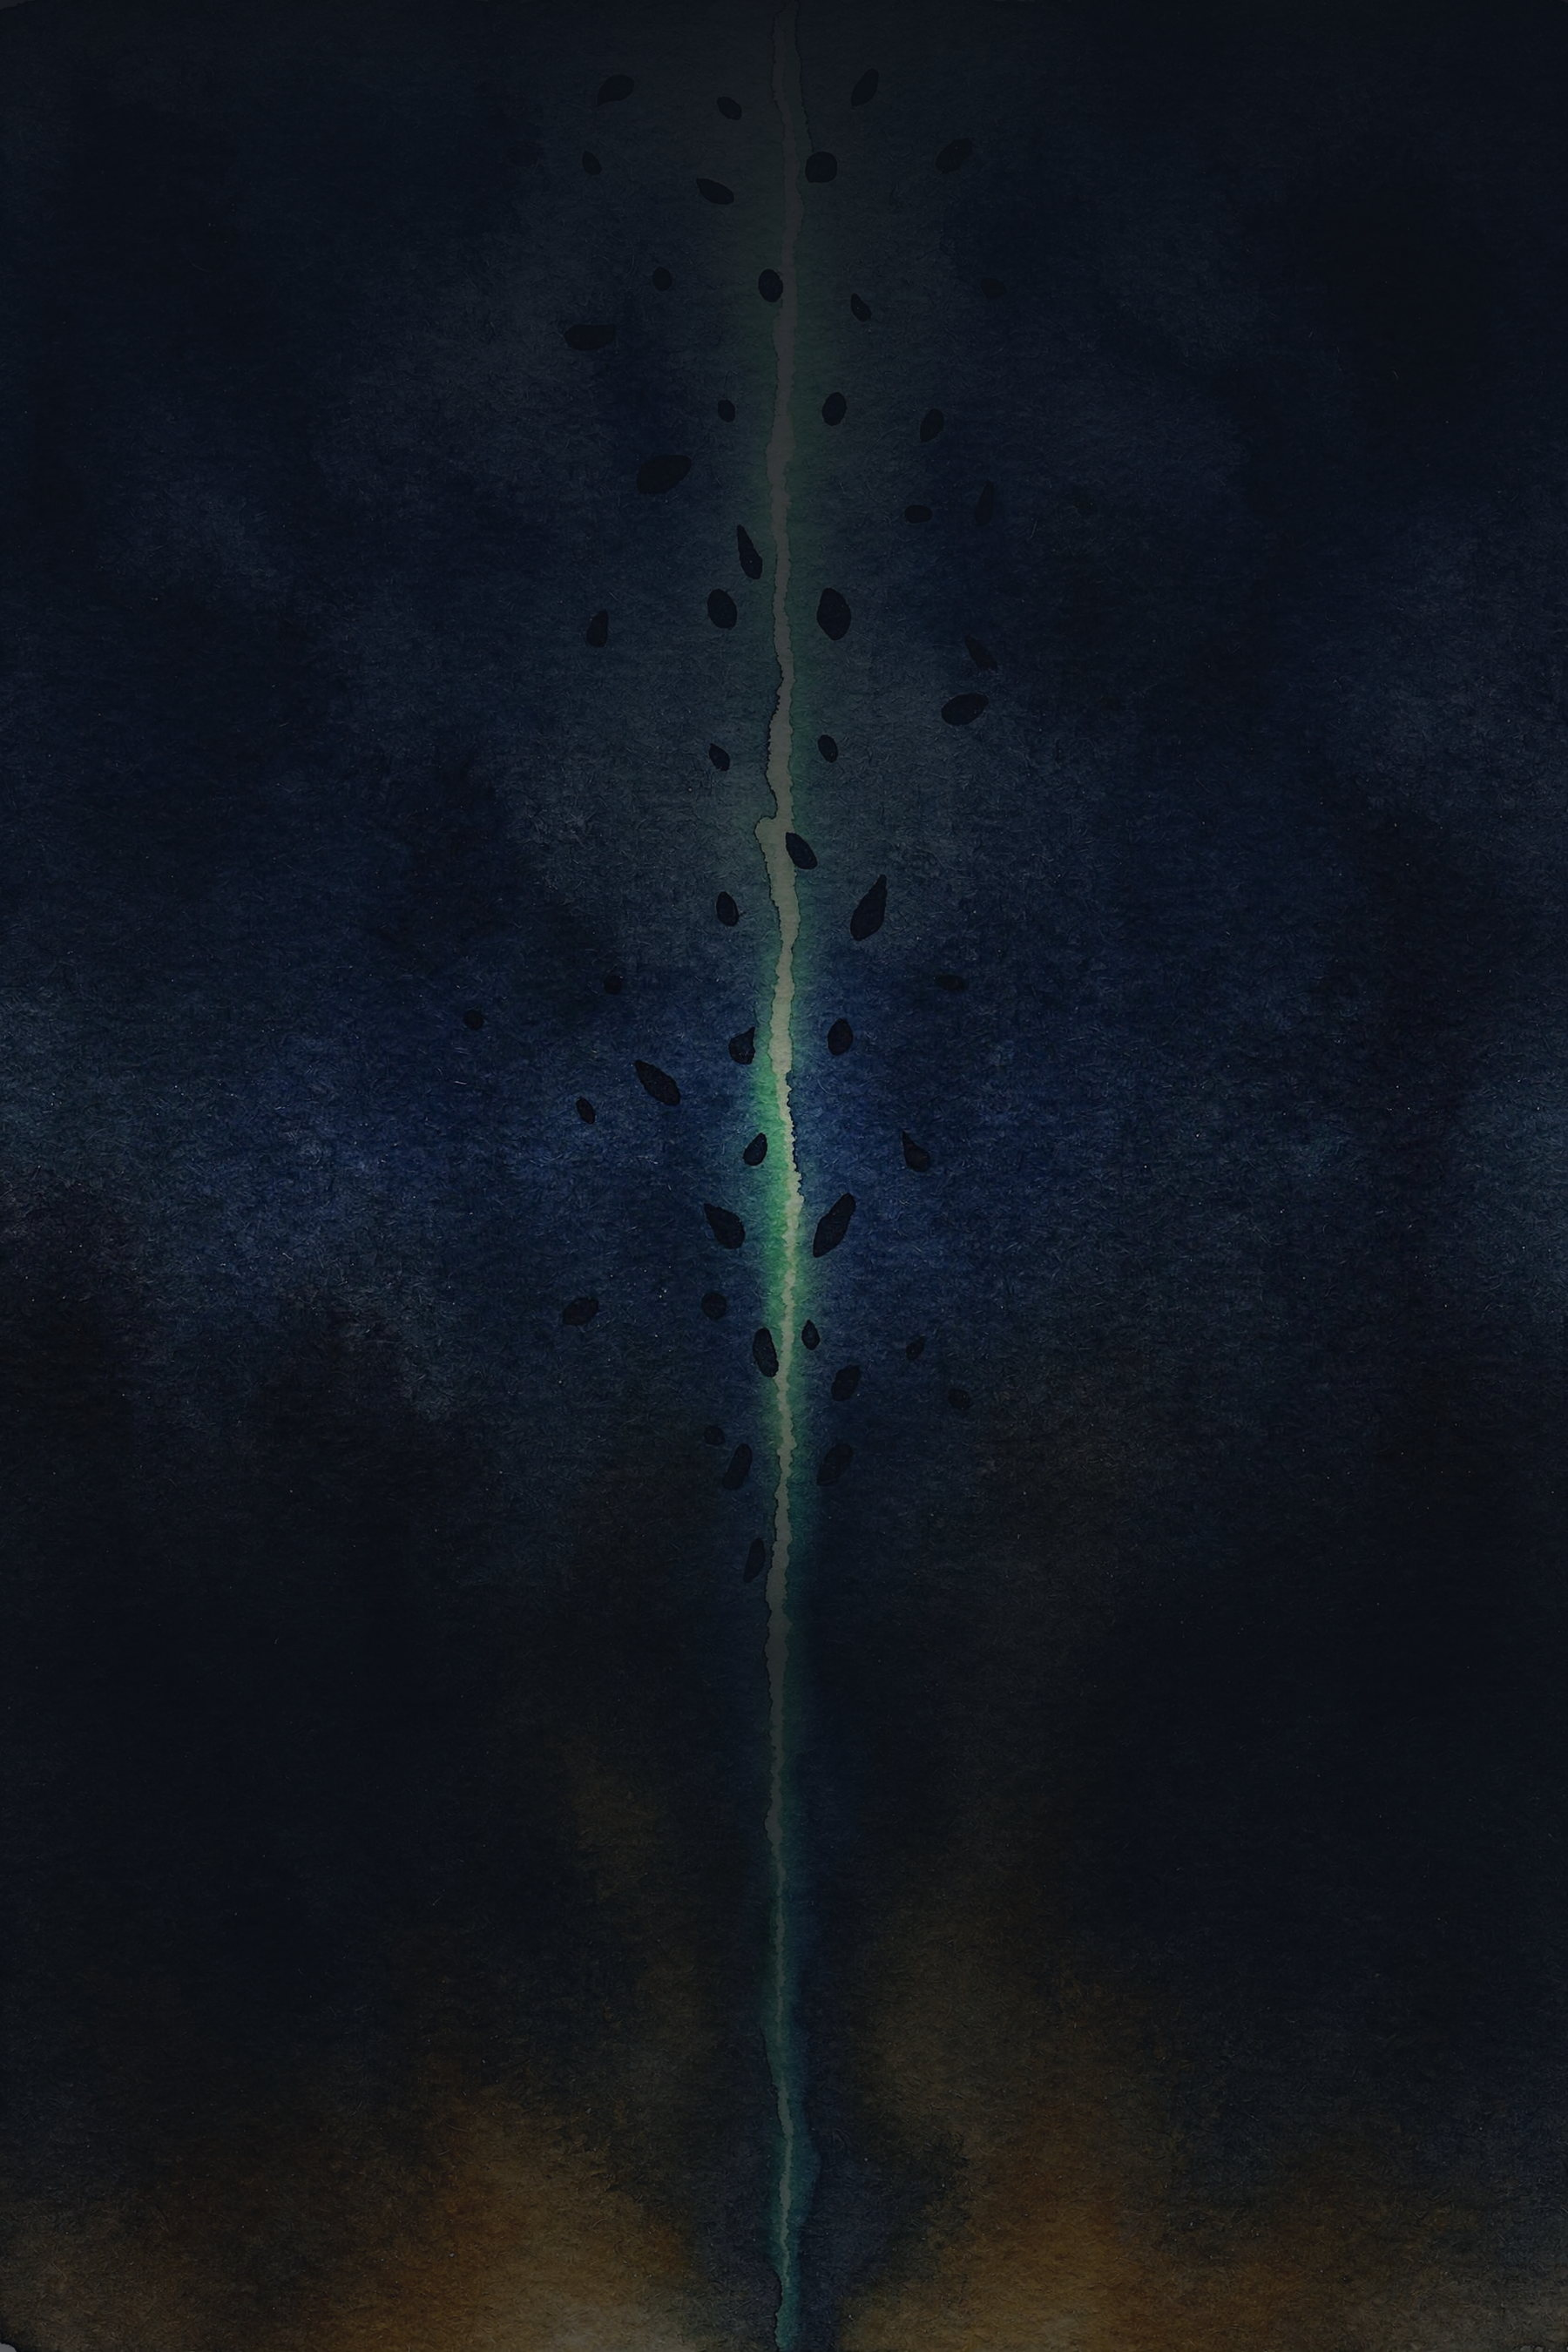
\includegraphics[width=\paperwidth,height=\paperheight]{../figures/cover_front_art.jpg}};



  % ---- identity block ----------------------------------------------------
  \node[anchor=south west,inner sep=0,text=accent] at ([xshift=0.60in,yshift=8.40in]current page.south west)
    {\fontsize{7.0}{8.4}\selectfont\sffamily
     \addfontfeatures{LetterSpace=18}A CRITICAL AUDIT OF A CLAIMED PROOF};

  \node[anchor=south west,inner sep=0,text=txt] at ([xshift=0.60in,yshift=7.74in]current page.south west)
    {\fontsize{33.5}{38}\selectfont\sffamily\bfseries IS THE RIEMANN};

  \node[anchor=south west,inner sep=0,text=txt] at ([xshift=0.60in,yshift=7.265in]current page.south west)
    {\fontsize{33.5}{38}\selectfont\sffamily\bfseries HYPOTHESIS};

  \node[anchor=south west,inner sep=0,text=accent] at ([xshift=0.60in,yshift=6.79in]current page.south west)
    {\fontsize{33.5}{38}\selectfont\sffamily\bfseries SOLVED?};

  \fill[accent] ([xshift=0.60in,yshift=6.40in]current page.south west)
         rectangle ([xshift=5.48in,yshift=6.43in]current page.south west);

  \node[anchor=south west,inner sep=0,text=txt,align=left] at ([xshift=0.60in,yshift=5.66in]current page.south west)
    {\fontsize{10.4}{13}\selectfont\sffamily
     A Critical Audit of the Lean Formalization,\\
     the Theta-Lift Method, and the\\
     Two-Thirds Ceiling};

  \node[anchor=south west,inner sep=0,text=dim,align=left] at ([xshift=0.60in,yshift=5.27in]current page.south west)
    {\fontsize{9.4}{13.5}\selectfont\sffamily\itshape
     It compiles. It has no axioms.\\
     Nobody has checked the mathematics.};

  % ---- credits -----------------------------------------------------------
  \node[anchor=south west,inner sep=0,text=accent] at ([xshift=0.60in,yshift=2.60in]current page.south west)
    {\fontsize{8.4}{10}\selectfont\sffamily On the mathematics of Levent Alpöge};

  \node[anchor=south west,inner sep=0,text=txt] at ([xshift=0.60in,yshift=2.38in]current page.south west)
    {\fontsize{12.2}{14}\selectfont\sffamily\bfseries GERALD ENRIQUE};

  \node[anchor=south west,inner sep=0,text=txt] at ([xshift=0.60in,yshift=2.175in]current page.south west)
    {\fontsize{12.2}{14}\selectfont\sffamily\bfseries NELSON MC KENZIE};

  \fill[accent] ([xshift=0.60in,yshift=1.915in]current page.south west)
         rectangle ([xshift=1.16in,yshift=1.938in]current page.south west);

  \node[anchor=south west,inner sep=0,text=dim,align=left] at ([xshift=0.60in,yshift=1.14in]current page.south west)
    {\fontsize{8.4}{11.8}\selectfont\sffamily
     Tico Internet LLC\\
     2026 First Edition\\
     Licensed under the Apache License 2.0\\
     DOI 10.5281/zenodo.24408811};
\end{tikzpicture}
\null
\end{document}
